\chapter{Segmentation methods based on Intensity Discontinuity(edge detection)}
Segmentation techniques based on Intensity Discontinuity are used to detect the boundary of the system and clearly if the boundary is closed then that boundary defines a region i.e the pixels that are inside the boundary.

\begin{figure}[h!]
  \centering
  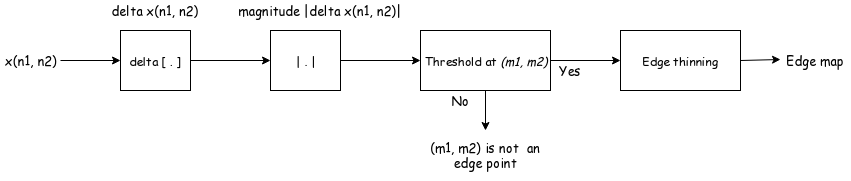
\includegraphics[width=15cm,height=6cm,keepaspectratio]{img/edge_detection_block.png}
  \caption{edge detection block diagram}
\end{figure}
Above figure is basic building block of edge detection algorithm. $x(n_1,n_2)$ is an input image of which the edges we need to find. The gradient for this image is what needs to be found, so at this point we have available a 2D array and
each entry of the array is a vector. After this step the magnitude of the gradient is found and exactly at this point we discard the directionality of the edges and just keep its strength so now we have the length of the vector and each entry in the 2D array is a scalar. Next, the numbers in the array are compared against the threshold. If the number at location for e.g $(m_1,m_2)$ is smaller than the threshold, then no edge exists at that point. If, however, the value's greater than the threshold, then $(m1, m2)$ pixel belongs to an edge. Since identifying edge pixels is based on this thresholding operation, very often it ends up with thick edges. Edges, multiple pixels belonging to an edge and therefore typically an edge thinning algorithm.  As the name implies, the width of those edges are thinned, thus they becomes smaller, maybe a couple of pixels and finallly we have the edge map of the original image $x(n_1, n_2)$.
\section{Sobel Operator}\index{Sobel Operator}
Sobel operator is a gradient operator which has emphasis in edge detection in images. It is basically a convolution filter of mask
size \texttt{2 x 2}, \texttt{3 x 3} which is used to compute image derivative. It has a separable properties. Sobel operator is good at detecting stronger edges but the weaker edges are faint and disappear after thresholding.

\subsection{Image \texttt{group\_of\_coins}}
We executed Sobel operator on this image. The process starts by turning the color image into graylevel image followed by smoothening image using a gaussian filter with standard deviation of 1.0. After this, we extract the threshold value of the image used by sobel operator. Then we multiply the initial threshold value by \texttt{fudge\_fx} which holds float value and run the sobel operator on that image again which indeed gives us the best of what sobel operator has to offer.
The end result give us just 2 complete boundary of coins while the rest are incomplete boundaries. We discuss a remedy for solving this problem in the summary section.

\subsection{Image \texttt{another\_group\_of\_coins}}
For this image we applied the same step as the previous image. The end result is also incomplete boundaries which we address the same in the summary section.

\subsection{Image \texttt{pillars\_of\_hercules}}
For this image, the only change is to adjust \texttt{fudge\_fx} set to 0.7 to get the desired outcome.

\section{Canny Edge Detector}\index{Canny Edge Detector}
Canny Edge detector does better \textbf{edge linking} compared to sobel operator. The four fundamental steps of canny edge detector are -
\textbf{Canny Edge Algorithm}
\begin{enumerate}
  \item Smooth the image using gaussian filter $\sigma$.
  \item compute the gradient magnitude and angle images.
  \item apply non-maximal suppression to the gradient magnitude image.
    \begin{enumerate}
    \item let $d_1$,$d_2$,$d_3$,$d_4$ be four basic edge directions(horizontal, -45 degrees, +45 degress, vertical).
    \item At every point $(n_1, n_2)$ in $\alpha(n_1, n_2)$:
      \begin{enumerate}
      \item find the direction $d_k$ that is closest to $\alpha(n_1, n_2)$
        \item if the value of $M(n_1, n_2)$ is less then at least one of its neighbors along $d_k$, ignore/supress it or else keep it.
      \end{enumerate}
    \end{enumerate}
  \item finally use double thresholding $(T_H, T_L)$.
    \begin{enumerate}
      \item Pixels with values greater than $T_H$ are strong edge pixels
        \item Pixels with value smaller than $t_L$ are weak edge pixels
    \end{enumerate}
  \item perform edge linking
    \begin{enumerate}
      \item Locate a pixel $p$ belonging to a strong edge
      \item Find weak pixels that are connected to $p$
      \item append these weak pixels to $p$
    \end{enumerate}
\end{enumerate}

\subsection{Image \texttt{group\_of\_coins}}
The process remains the same as discussed previously. The only difference is we use canny edge algorithm in place of sobel and set the fudge value to 0.6. The end result is much improved than sobel result.

\subsection{Image \texttt{pillars\_of\_hercules}}
For this image we have set the fudge value to .9. There are still some incomplete edge lines which need attention. The solution is discussed in summary section of the report.

\chapter{Morphological Operation}\index{Morphological Operation}
Morphological Operation is another technique for image segmentation. It consist of \textbf{erosion}, \textbf{dilation}, \textbf{opening}, \textbf{closing} operations, also, but important, \textbf{skeletonization}.

\subsection{Image \texttt{baby\_elephant}}
First I binarize the image and then invert it. Then I make use of \textbf{erosion} to erode the surroundings, then we use \texttt{getsinglepixel} function to eliminate miniature isolated pixels. The process is still not complete. Futher we use \texttt{bpropagation} to allow constraint dilation. Futher, using \texttt{bskeleton} through the use of \textit{looseendsaway} we isolate regions of the image and then use branch pixels to get the main object. The final result is elimination of background pixel thus focusing on foreground object. This is best we can get using morphology.
\chapter{Edge detection using maximum filter}\index{Edge detection using maximum filter}
Maximum filter can also be used for edge detection outcome. Like erosion in morphology operation, maximum filter erodes shapes on the image.

\subsection{Image \texttt{group\_of\_coins}}
For this image, I apply unsharpening mask and then perform image subtraction from the result of maximum filter and result of unsharpen mask

\subsection{Image \texttt{another\_coins}}
The process is exactly the same as the maximum filter used for group of coins
%%% Local Variables:
%%% mode: latex
%%% TeX-master: t
%%% End:
